\documentclass{article}
\usepackage{tikz}
\usepackage{tkz-euclide} % loads  TikZ and tkz-base
\usetkzobj{all}
\usetikzlibrary{calc,math}
\begin{document}
	
	
	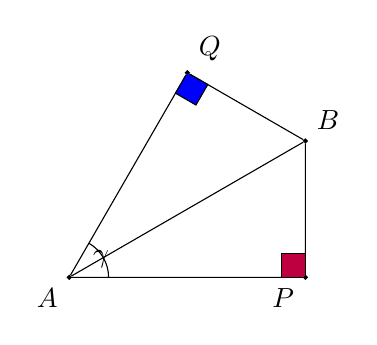
\begin{tikzpicture}
	[scale=1,>=stealth,point/.style={draw,circle,fill = black,inner sep=0.5pt},]
	


	
	\node (A) at (0,0)[point,label=below left:$A$] {};
	\node (P) at (3, 0)[point,label=below left:$P$] {};
	%\node (Q) at ($({3*\cos{60}}, {3*\sin{60}})$)[point,label=below right:$Q$] {};
	%\node (B) at ($({3.4641*\cos{30}}, {3.4641*\sin{30}})$)[point,label=above right:$B$] {};
		\node (Q) at (1.5, 2.598)[point,label=above right:$Q$] {};
	\node (B) at (3, 1.732)[point,label=above right:$B$] {};
	
	
	
	
	\draw (A) -- node[left] {$\textrm{}$} (P) -- node[below] {$\textrm{}$} (B) -- node[above,xshift=2mm] {$\textrm{}$} (Q);
	\draw (A)--(Q);
	\draw (A)--(B);
	
	
	
	\tkzMarkAngle[fill=orange!40,size=0.5cm,mark=](P,A,Q)
	 \tkzMarkRightAngle[fill=blue,size=.3](A,Q,B);
	 \tkzMarkRightAngle[fill=purple,size=.3](A,P,B);
	%\tkzMarkRightAngle[fill=orange!40,size=0.4cm,mark=](A,Q,B)
	%\tkzMarkRightAngle[fill=green!40,size=0.5cm,mark=](A,P,B)
	
	\tkzLabelAngle[pos=0.45](P,A,Q){$\gamma$}
	
	\end{tikzpicture}
	


\end{document}
